\documentclass[conference]{IEEEtran}
\IEEEoverridecommandlockouts
% The preceding line is only needed to identify funding in the first footnote. If that is unneeded, please comment it out.
\usepackage{cite}
\usepackage{amsmath,amssymb,amsfonts}
\usepackage{algorithmic}
\usepackage{graphicx}
\usepackage{textcomp}
\usepackage{xcolor}
\usepackage{tabularx}
\usepackage{multirow}
\usepackage{graphics} % for pdf, bitmapped graphics files
\usepackage{subfig}
\usepackage{subcaption}
\usepackage{hyperref}
\usepackage{academicons}
\usepackage{xcolor}
\usepackage{listings}
\usepackage{tabularx} % Asegúrate de incluir este paquete

\usepackage{tikz}
\usetikzlibrary{shapes.geometric, arrows}

\usetikzlibrary{shapes.geometric, arrows}

\tikzstyle{startstop} = [rectangle, rounded corners, minimum width=3cm, minimum height=1cm,text centered, draw=black, fill=red!30]
\tikzstyle{process} = [rectangle, minimum width=3cm, minimum height=1cm, text centered, draw=black, fill=blue!30]
\tikzstyle{arrow} = [thick,->,>=stealth]


\def\BibTeX{{\rm B\kern-.05em{\sc i\kern-.025em b}\kern-.08em
		T\kern-.1667em\lower.7ex\hbox{E}\kern-.125emX}}

% Color Enlace
\definecolor{colorEnlace}{RGB}{0, 0, 0}
\hypersetup{
	colorlinks=true,
	linkcolor=colorEnlace,
	citecolor=colorEnlace,
	urlcolor=colorEnlace,
	pdfauthor={Davis Bremdow Salazar Roa},
	pdftitle={Sistemas Embebidos}
}
\definecolor{mybg}{rgb}{0.97,0.97,0.97}
\definecolor{mygray}{gray}{0.4}
\definecolor{mygreen}{rgb}{0,0.6,0}
\definecolor{myblue}{rgb}{0,0,0.8}
\definecolor{mypurple}{rgb}{0.58,0,0.82}
\definecolor{myred}{rgb}{0.7,0,0}

\lstdefinelanguage{MatlabEnhanced}{
	language=Matlab,
	morekeywords={[2]linspace,plot,title,xlabel,ylabel,legend,grid},
	morekeywords={[3]sin,cos,exp,log,sqrt},
	keywordstyle=\color{myblue}\bfseries,
	keywordstyle=[2]\color{mypurple},
	keywordstyle=[3]\color{myred},
	commentstyle=\color{mygreen}\itshape,
	stringstyle=\color{mygray},
	morecomment=[l]%
}

\lstset{
	language=MatlabEnhanced,
	backgroundcolor=\color{mybg},
	frame=single,
	basicstyle=\ttfamily\small,
	showstringspaces=false,
	numbers=none,              %
	xleftmargin=0pt,           %
	framexleftmargin=0pt,      
	framexrightmargin=0pt,
	framextopmargin=2pt,
	framexbottommargin=2pt,
	breaklines=true,
	tabsize=1,
}

% Control 
\usepackage{amsmath}
\begin{document}
	
	\title{Informe final - Amplificador Diferencial Retroalimentado}
	\author{
		\makebox[\textwidth][c]{\large\textbf{Universidad Nacional de San Antonio Abad del Cusco}}\\
		\makebox[\textwidth][c]{\normalsize\textit{Escuela profesional de Ingeniería Electrónica}}\\
		\makebox[\textwidth][c]{\normalsize\textit{Telecomunicaciones I}}\\
		\and
		\IEEEauthorblockN{Ing. Milton Velasquez Curo}
		\IEEEauthorblockA{Ingeniero Electrónico \\
			Cusco, Perú \\
			milton.velasquez@unsaac.edu.pe}
		\and
		\IEEEauthorblockN{Ruth Juana Espino Puma - 185746}
		\IEEEauthorblockA{Estudiante de Ingeniería Electrónica \\
			Cusco, Perú \\
			184657@unsaac.edu.pe}
		\and
		\IEEEauthorblockN{Davis Bremdow Salazar Roa - 200353}
		\IEEEauthorblockA{Estudiante de Ingeniería Electrónica \\
			Cusco, Perú \\
			200353@unsaac.edu.pe}
	}
	
	\maketitle
	\begin{abstract}
		La modulación es un proceso fundamental en las telecomunicaciones que consiste en variar una o más propiedades de una señal portadora (como amplitud, frecuencia o fase) en función de una señal de información o mensaje. Este proceso permite transmitir información a largas distancias de manera eficiente, minimizando interferencias y aprovechando mejor el espectro de frecuencias. Existen varios tipos de modulación, entre ellos la modulación en amplitud (AM), frecuencia (FM) y fase (PM), cada una con características y usos específicos según las necesidades del sistema de comunicación.
		
		El índice de modulación es una medida que cuantifica la variación de la señal portadora en relación con la señal moduladora. Su importancia radica en que determina la eficiencia espectral, la calidad de la señal transmitida y el nivel de distorsión. Un índice bajo puede resultar en una señal débil o difícil de demodular, mientras que un índice muy alto puede causar sobre modulación y distorsión. En aplicaciones prácticas, la modulación es utilizada en radiodifusión (radio y televisión), comunicaciones satelitales, telefonía móvil, redes Wi-Fi, y sistemas de control industrial, donde el índice de modulación debe ser cuidadosamente ajustado para garantizar un rendimiento óptimo.
	\end{abstract}
	
	\begin{IEEEkeywords}
		Modulación, portadora, señal, índice de modulación, amplitud, frecuencia, fase, transmisión, espectro, distorsión.
	\end{IEEEkeywords}
	
	%% TODO: Contenido del documento
	
	\section{Modulación DSB - SC}
	
	\section{Modulación SSB}
	\subsection{\textbf{Generación de una USB}}
	
	La generación de una señal modulada SSB (Single Side Band) esta definida en función a la ecuación \ref{eq:generacion-ssb} en la cual se definen 2 señales sinusoidales que hacen de portadoras y la moduladora la cual esta relacionada con su equivalente luego de aplicar la transformada de Hilbert y la cual se multiplicara por la señal portadora desfasada 90º.
	
	\begin{equation}
		s_{SSB}(t) = \frac{A_e}{2}m(t)\cos(2\pi f_c t) \mp \frac{A_e}{2}\hat{m}(t)\sin(2\pi f_c t)
		\label{eq:generacion-ssb}
	\end{equation}
	
	\subsection{\textbf{Generación una USB en MATLAB}}
	
	Para la generación computacional de este tipo de modulación en MATLAB es necesario definir todas sus componentes siendo el caso que para la generación de una señal SSB - USB tan solo es necesario definir la resta en la ecuación \ref{eq:generacion-ssb}.
	
	A forma de ejemplo el código matlab para ello se muestra en el listing \ref{lst:generacion-ssb}
	\begin{lstlisting}[caption="asdf", label="lst:generacion-ssb"]
		%% CONFIGURACION INICIAL
		clc; clear; close all;
		fs = 100000;                 % Frecuencia de muestreo
		t = 0:1/fs:0.1-1/fs;         % Vector de tiempo (100 ms)
		N = length(t);               % Numero de muestras
		
		%% PARAMETROS DE SENALES
		% Portadora
		fc = 1000;                   % Frecuencia portadora
		Ac = 1;                      % Amplitud portadora
		
		% Moduladora (mensaje)
		fm = 100;                    % Frecuencia mensaje
		Am = 1;                      % Amplitud mensaje
		m = Am*cos(2*pi*fm*t);       % Senal moduladora
		
		%% GENERACION DE SENALES
		% Portadora
		c = Ac*cos(2*pi*fc*t);
		
		% DSB-SC
		dsb_sc = m .* c;
		
		% SSB (Metodo de filtrado)
		filtro_pb = fir1(100, fm/fs);  % Filtro pasa bajos
		hilbert_m = imag(hilbert(m));   % Transformada de Hilbert
		ssb_usb = (m.*cos(2*pi*fc*t) - (hilbert_m.*sin(2*pi*fc*t)));
		ssb_usb = filter(filtro_pb, 1, ssb_usb); % Filtrado final
	\end{lstlisting}
	
	Siendo así que el único cambio a realizar en el equivalente digital para la generación de la señal SSB es el cambio de signo en la ecuación que genera este tipo de modulación.
	
	\subsection{\textbf{Análisis del espectro para LSB y USB}}
	
	En las figuras \ref{fig:modulacion-lsb} y \ref{fig:modulacion-usb} se pueden apreciar el espectro de una señal SSB - LSB y una SSB - USB respectivamente y en las cuales se pueden destacar que al igual que en otros tipos de modulación se tiene el desplazamiento en frecuencia con la diferencia que para este tipo de modulación solo se hace uso de una banda lateral ya sea la inferior o superior
	
	\begin{figure}[h]
		\centering
		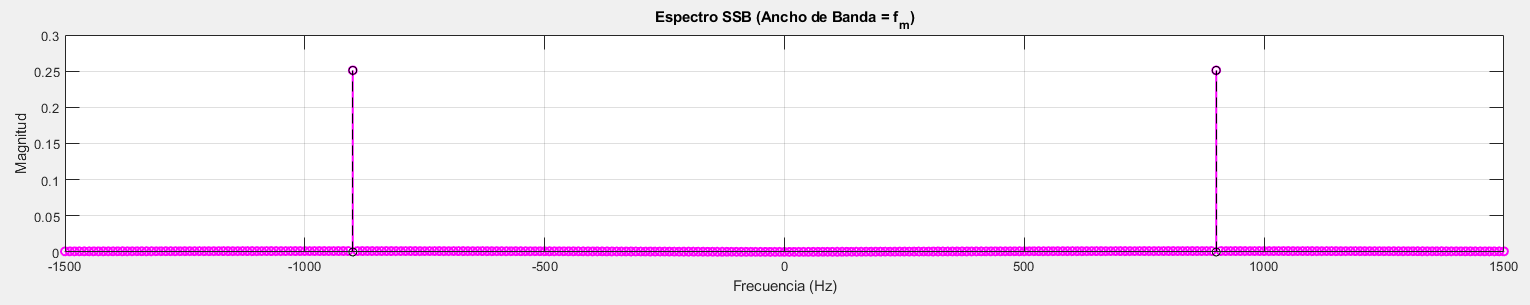
\includegraphics[width=0.5\textwidth]{media/modulacion-lsb}
		\caption{Espectro de una señal SSB - LSB}
		\label{fig:modulacion-lsb}
	\end{figure}
	
	\begin{figure}[h]
		\centering
		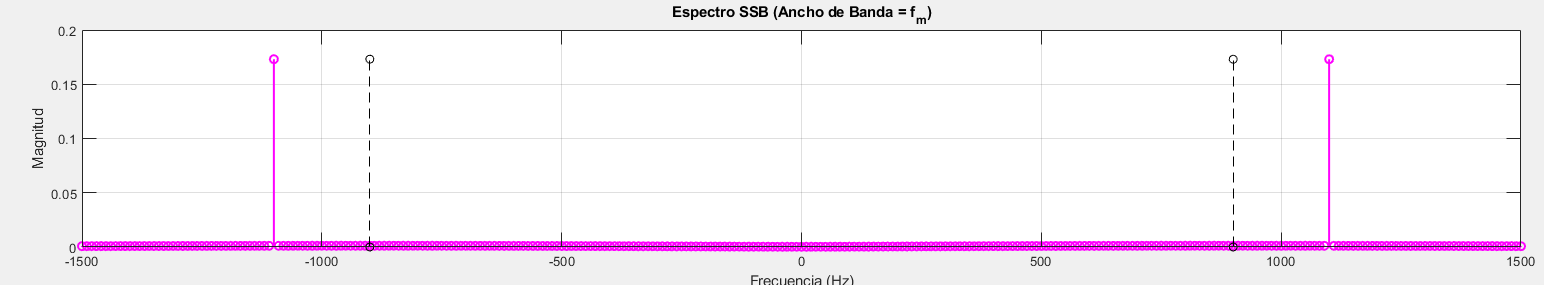
\includegraphics[width=0.5\textwidth]{media/modulacion-usb}
		\caption{Espectro de una señal SSB - USB}
		\label{fig:modulacion-usb}
	\end{figure}	
	
	\section{Generación de una SSB mediante el método del filtrado}
	Otra forma de poder generar una señal SSB es mediante el empleo de un filtro pasa altos con el cual se elimine una de las bandas laterales, para ello se puede hacer uso de una modulación DSB - SC y luego aplicar un filtro pasa alto en la frecuencia desplaza inferior o superior para la generación de la señal SSB, siendo este proceso el que se apreciar en al figura \ref{fig:}
	
	\begin{figure}[h]
		\centering
		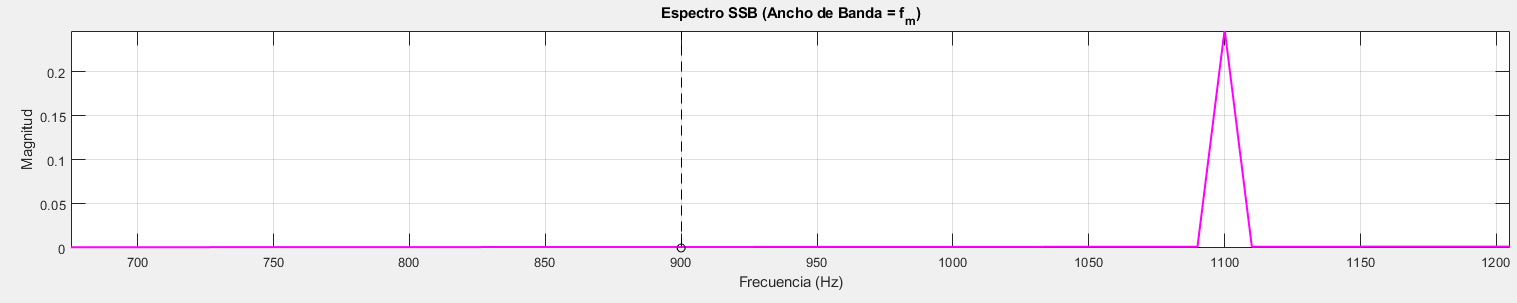
\includegraphics[width=0.5\linewidth]{media/generacion-usb}
		\caption{Generación una señal SSB - USB mediante el método del filtrado}
		\label{fig:generacion-usb}
	\end{figure}
	
	\section{Ventajas de una modulación SSB frente a una DSB-SC}
	
	La principal ventaja de la modulación de banda lateral única (SSB) es que ocupa la mitad del ancho de banda, lo que permite una mayor eficiencia espectral y mejor uso del canal asignado para la transmisión de más señales en un mismo rango de frecuencias; además, consume menos potencia al transmitir solo una banda lateral, lo que mejora la eficiencia energética sin sacrificar la calidad de la señal, mientras que en DSB-SC se desperdicia potencia al transmitir dos bandas laterales redundantes. Estas características hacen que SSB sea preferible en aplicaciones donde el ancho de banda y la potencia son limitados, como en comunicaciones por radio de onda corta o sistemas multiplexados.
	
	\section{Generación de una SSB - USB mediante diagrama de bloques}
	
	El diagrama de bloques y la secuencia de pasos realizados para la generación de una señal SSB se muestran en la figura \ref{fig:generacion-usb-bloques} en la cual se destaca el empleo de la modulación DSB - SC y luego de aplica un filtro pasa altos para recuperar solo la banda lateral superior.
	
	\begin{figure}[h]
		\centering
		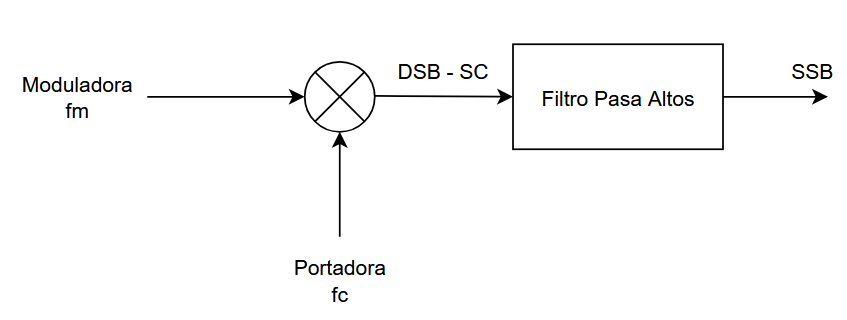
\includegraphics[width=0.4\textwidth]{media/generacion-usb-bloques}
		\caption{Generación de una SSB - USB mediante diagrama de blqoues}
		\label{fig:generacion-usb-bloques}
	\end{figure}
	
	\section{Cuestionario - Teórico}
	\subsection{\textbf{¿Por qué la modulación DSB - SC es más eficiente que AM convencional?}}
	La modulación DSB-SC (Double Sideband Suppressed Carrier) es más eficiente que la AM convencional porque elimina la portadora, la cual no transporta información pero consume la mayor parte de la potencia transmitida. Al suprimir la portadora, DSB-SC concentra toda la potencia en las bandas laterales, que contienen la información útil, lo que permite un uso más eficiente de la energía y reduce el consumo de potencia sin perder calidad en la señal.
	\subsection{\textbf{Explique el principio de funcionamiento del filtro de Hilbert}}
	El filtro de Hilbert es un procesador de señales que desplaza la fase de todas las componentes de frecuencia de una señal en -90 grados, sin alterar su amplitud. Su principio de funcionamiento se basa en crear una versión ortogonal de la señal original, lo que es útil en aplicaciones como la generación de señales analíticas (señales complejas sin componentes de frecuencia negativas) y en sistemas de modulación SSB (Banda Lateral Única), donde ayuda a eliminar una de las bandas laterales.
	\subsection{\textbf{¿Que ventajas tiene SSB sobre DSB-SC en aplicaciones practicas?}}
	La modulación SSB (Single Sideband) tiene ventajas prácticas sobre DSB-SC, principalmente porque ocupa la mitad del ancho de banda, lo que permite una mayor eficiencia espectral y la transmisión de más canales en un mismo rango de frecuencias. Además, SSB requiere menos potencia para transmitir la misma información, ya que solo envía una banda lateral y suprime tanto la portadora como la otra banda lateral, lo que la hace ideal para comunicaciones de larga distancia y sistemas con limitaciones de potencia.
	
	\section{Cuestionario - Ejercicios}
	
	\subsection{\textbf{Generación de una señal AM}}
	
	Considerando una portadora definida en \ref{eq:moduladora-ejercicio} se busca generar el espectro de la señal DSB - SC, el diseño del filtro para la obtención una señal SSB y el calculo del ancho de banda para ambos casos.
	
	\begin{equation}
		m(t) = 2\cos(2\pi 200t) + \cos(2\pi 300t)
		\label{eq:moduladora-ejercicio}
	\end{equation}
	
	Para definir el espectro de \ref{eq:moduladora-ejercicio} se debe analizar la señal moduladora la cual consta de 2 tonos de menor y mayor frecuencia, siendo la señal modulada resultante una combinación de 4 impulsos en la modulación DSB - SC como se apreciar en la figura \ref{fig:dsb-sc-ejercicio}
	
	\begin{figure}[h]
		\centering
		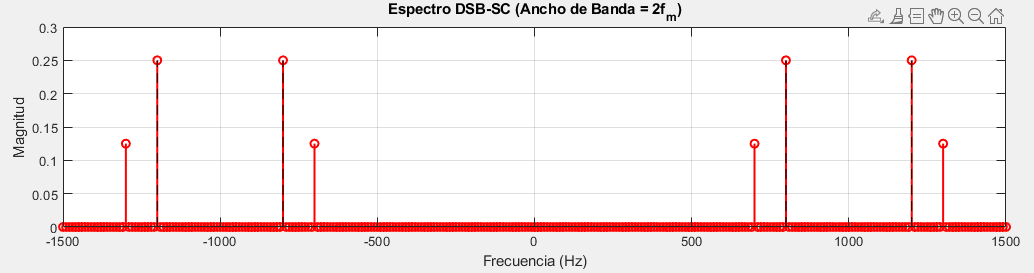
\includegraphics[width=0.5\textwidth]{media/dsb-sc-ejercicio}
		\caption{Señal DSB-SC generada}
		\label{fig:dsb-sc-ejercicio}
	\end{figure}
	
	Para el caso de la generación de una señal SSB - LSB es necesario definir un filtro pasa banda centrado en 850 Hz con un ancho de banda de 300 Hz para recuperar la banda lateral inferior, siendo el resultado de este proceso el que se muestra en al figura \ref{fig:ssb-ejercicio}
	
	\begin{figure}[h]
		\centering
		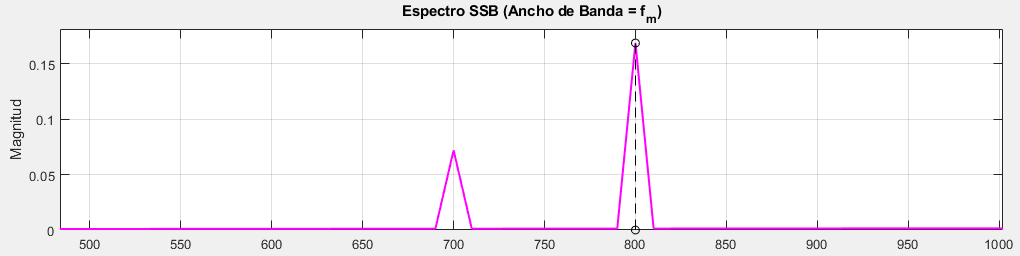
\includegraphics[width=0.5\textwidth]{media/ssb-ejercicio}
		\caption{Señal SSB - LSB mediante filtrado}
		\label{fig:ssb-ejercicio}
	\end{figure}
	
	Finalmente para el calculo del ancho de banda se debe enfatizar que este se encuentra en función del tipo de modulación a usar, siendo así que para una modulación DSB - SC como se define en \cite{tomasi2004sistemas} el ancho de banda será dos veces el ancho de banda de la señal de información y para una SSB se mantendrá el ancho de bana de la señal de información.
	
	Para una modulación DSB - SC el ancho de banda será:
	\begin{align*}
		DSB_{BW} &= 2fm \\
		DSB_{BW} &= 600
	\end{align*}
	
	Para una modulación SSB el ancho de banda será:
	
	\begin{align*}
		SSB_{BW} = fm \\
		SSB_{BW} = 300
	\end{align*}
	
	\section{Conclusiones}
	
	\begin{itemize}
		\item DSB-SC elimina la portadora mejorando eficiencia.
		\item SSB reduce el ancho de banda a la mitad.
		\item MATLAB permite visualizar claramente los efectos de cada técnica.
		\item El análisis espectral es fundamental para validar los resultados.
	\end{itemize}
	
	\bibliographystyle{IEEEtran}
	\bibliography{biblio}
\end{document}
